\chapter{Estados del juego}
Sin contar los niveles y las cinemáticas, el juego se compone de tres interfaces: Interfaz 1.00 (Ver interfaz \ref{inter:interfaz01}), correspondiente a la pantalla de inicio; la interfaz 2.00 (Ver interfaz \ref{inter:interfaz02}), que corresponde al menú principal; y la interza 3.00 (Ver interfaz \ref{inter:interfaz03}), correspondiente al menu de selección de nivel. Como se puede ver en la figura %%\ref{}  

Ver figura \ref{fig:EstadosJuego}
\begin{figure}
  \centering
     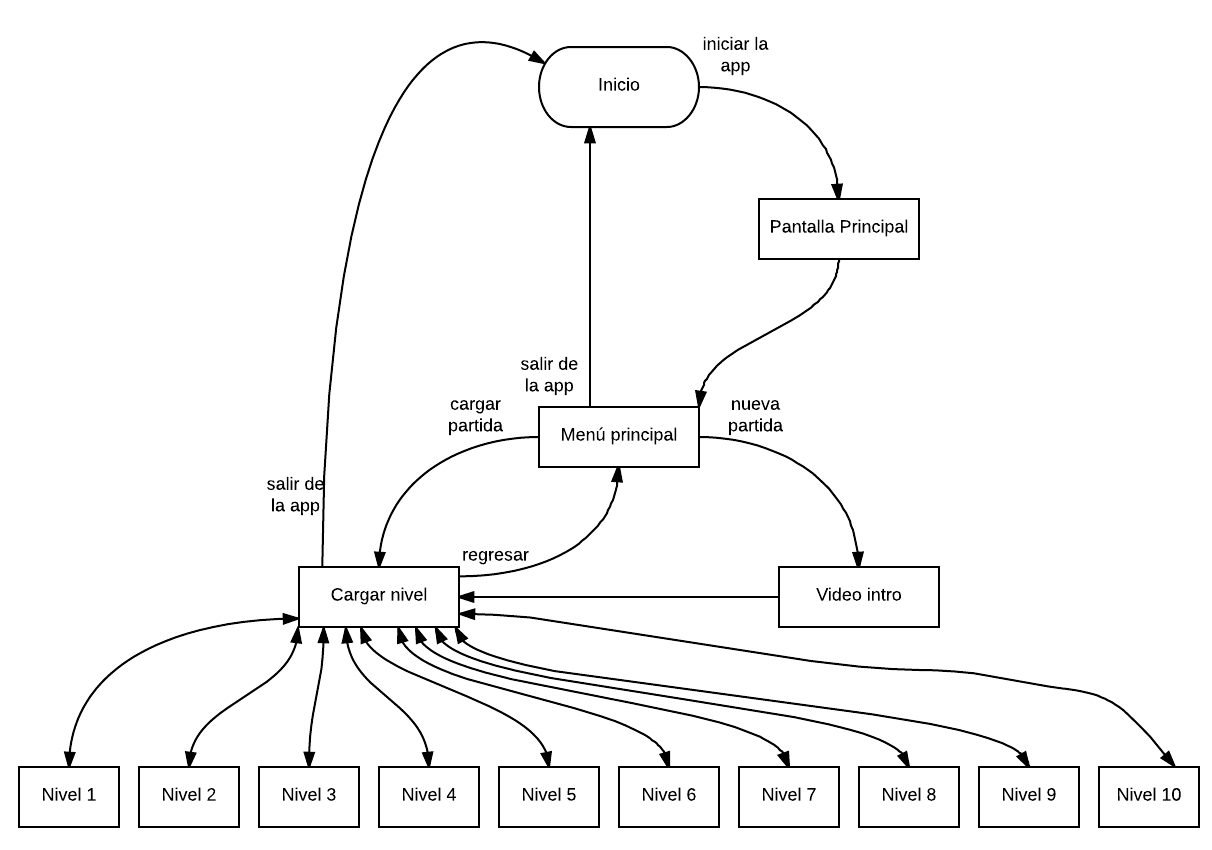
\includegraphics[width=\linewidth]{Imagenes/estadosJuego}
  \caption{Progreso del juego}
  \label{fig:EstadosJuego}
\end{figure}  